\documentclass[aspectratio=169,professionalfonts,10pt]{beamer}

\newbool{russian}
\booltrue{russian}  % Загружает русскоязычный логотип ВШЭ
\usepackage{HSE-theme/beamerthemeHSE}

\usepackage[english,russian]{babel}
\usepackage{unicode-math}

\usepackage{biblatex}
\addbibresource{bibliography.bib}

\setmainfont{HSE Sans}
\setsansfont{HSE Sans}
\setmathrm[Numbers={Lining,Proportional}]{HSE Sans}
\usepackage[scaled=0.8]{FiraMono}

\graphicspath{{images/}}  	% Папка с картинками

\usepackage{tikz}
\usepackage{listings}
\usepackage{tcolorbox}

\lstset{
  language=[LaTeX]TeX,
  basicstyle=\ttfamily,
  columns=fullflexible,
  keepspaces=true
}

\title[Сервис для индексирования и просмотра Git-репозиториев]{Сервис для индексирования и просмотра Git-репозиториев}
\subtitle{Git Repository Indexing and Viewing Service}
\author[Илья Коннов]{
    \begin{tabular}{r l}
        Выполнил
            & \textbf{Коннов Илья Александрович} \\
            & {\scriptsize студент группы БПИ201 образовтальной программы 09.03.04 «Программная инженерия»} \\
        Руководитель:
            & \textbf{Павлочев Николай Александрович} \\
            & {\scriptsize старший преподаватель, академический руководитель ОП «Программная инженерия»} \\
        Соруководитель:
            & \textbf{Топтунов Александр Алексеевич} \\
            & {\scriptsize приглашенный преподаватель департамента программной инженерии, ФКН}
    \end{tabular}
}
\institute[ФКН, ОП «Программная инженерия»]{Факультет компьютерных наук, департамент программной инженерии}
\date{2024}

\begin{document}	% Начало презентации

\frame[plain]{\titlepage}	% Титульный слайд

\section{Предметная область}
\begin{frame}{\insertsection}

При разработке ПО часто приходится читать чужой код многих разных проектов.

Для этого нужно иметь удобный интерфейс, которым легко пользоваться и который быстро работает.

При этом интерфейс должен помогать разработчику навигироваться по коду и давать подсказки.

\hfill

Этот проект посвящен изучению методов индексации кода и затем создания системы, которая бы предоставляла такой веб-интерфейс, в котором пользователь может использовать результаты индексации для облегчения чтения кода.

\end{frame}

\section{Основные термины, понятия и определения}
\begin{frame}{\insertsection}

\begin{itemize}
    \item \textbf{LSP} (Language Server Protocol) \cite{languageserver} — разработанный Microsoft протокол, позволяющий языковому серверу предоставлять редактору кода дополнительную информацию о \textbf{символах}.
    \item \textbf{Символ} (в контексте исходного кода) — идентифкатор в тексте программе, однажды где-либо определенный. Например, в строке «\texttt{def func():}» символом будет являться «func». Также символами являются имена переменных, классов и многое другое.
\end{itemize}

\end{frame}

\section{Актуальность}
\begin{frame}{\insertsection}

Многие компании так или иначе решают проблему просмотра и навигации по коду:

\begin{itemize}
    \item \textbf{GitHub}
        — разрабатывал механизм индексации с 2021 года и окончательно в 2023 сделал его доступным для всех репозиториев \cite{github-codesearch}.
    \item \textbf{Google}
        — активно разрабатывает и применяет приватный инструмент CodeSearch. Публично доступы инсталлцяции для просмотра проектов Chromium и Android (\cite{cs-chromium}, \cite{cs-android})
    \item \textbf{Facebook}
        — в разработке находится система Glean \cite{facebook-Glean}, также решающая задачу хранения информации о коде и связях между символами.
    \item \textbf{SourceGraph} \cite{sourcegraph}
        — разрабатывает коммерческий продукт для предоставления аналогичной функциональности своим пользователям.
\end{itemize}

\end{frame}

\section{Цель и задачи ВКР}
\begin{frame}{\insertsection}

\textbf{Цель работы} — разработать систему, позволяющая просматривать ранее проиндексированный репозиторий, при этом предоставляя инструменты навигации по нему.

\textbf{Задачи}:
\begin{enumerate}
    \item Разработать механизм получения файлов и директорий из Git-репозитория;
    \item Найти способ получать информацию о символах в коде и их связях, причем с поддержкой различных языков программирования;
    \item Разработать интерфейс для просмотра репозитория
    \item Разработать механизм отображения семантической информации в интерфейсе;
    \item Сделать простой способ развертывания и использования системы;
\end{enumerate}

\end{frame}

\section{Анализ существующих решений}
\begin{frame}{\insertsection}

Большинство найденных на момент аналогичных инструментов обладают теми или иными недостатками.

\begin{itemize}
    \item Большое количество инструментов поддерживает только отдельные языки (например, The Elixir Cross Referencer \cite{elixir-crossreferencer} для C/C++, SourceBrowser \cite{SourceBrowser} для .NET и многие другие)
    \item Применяющиеся в частных компаниях инструменты (Google, Яндекс, Facebook), обычно не доступны публично и часто об их существовании известно только из общения с сотрудниками.
    \item SourceGraph \cite{sourcegraph} — эффективно решает все индексации и навигации проблемы, но на данный момент больше не является открытым и бесплатным решением.
\end{itemize}

\end{frame}

\section{Функциональные требования}
\begin{frame}{\insertsection}

\begin{enumerate}
    \item Система должна иметь открытый исходный код и распространяться под свободной лицензией;
    \item Система должна иметь возможность индексирвать код на различных языках программирования. Обязательно должны поддерживаться языки Go, Rust, TypeScript и Kotlin;
    \item Система должна предоставлять функционал поиска определения символа, поиска всех использований символа и отображение справочной информации при наведении курсора на символ;
    \item Система должна иметь веб-интерфейс, в котором пользователь сможет просматривать содержимое репозитория;
    \item Система должна быть простой в развертывании и использовании;
    \item Система должна иметь возможность ограниченно использовать индексы построенные с использованием предыдущей версии репозитория даже при просмотре той версии, которая ещё не была проиндексирована.
\end{enumerate}

\end{frame}

\section{Метод получения файлов и директорий репозитория}
\begin{frame}[fragile=singleslide]{\insertsection}
Первая задача проекта — импортировать код Git-репозитория в систему.\\[2\baselineskip]

\begin{columns}
    \begin{column}{0.3\textwidth}
\begin{verbatim}
/repo/
├── source.c
└── .git/
    └── objects/
        ├── aa/aaaa…
        └── ...
\end{verbatim}
    \end{column}
    \begin{column}{0.7\textwidth}
        Можно читать напрямую файлы из директории с репозиторием. Это не будет работать с bare-репозиториями (например, на сервере) и не гарантирует, что файлы находятся под управлением Git.
        
        В этом проекте структура файлов и директорий считывается напрямую из объектов Git.
        
        Это позволяет сразу пропускать загрузку неизменных объектов, потому что идентифкатор объекта в системе Git зависит только от его содержимого.
    \end{column}
\end{columns}

\end{frame}

\section{Реализация пользовательского интерфейса}
\begin{frame}{\insertsection}

В качестве инструмента для просмотра кода используется Visual Studio Code \cite{vscode}. Этот редактор кода обладает ключевыми преимуществами:
\begin{itemize}
    \item Качественная реализация подсветки кода
    \item Возможность запускать в браузере без установки на компьютер
    \item Поддержка расширений, реализующих виртуальную файловую систему
    \item А также расширений, предоставляющие такой функционал как «перейти к определению» или справку при наведении курсора
\end{itemize}

Это позволяет сделать веб-интерфейс, отображающий файлы с сервера и одновременно с всеми требуемыми в проекте подсказками.

\end{frame}

\section{Метод получения данных индексации}
\begin{frame}{\insertsection}

Существует несколько инструментов индексации проектов:
\begin{itemize}
    \item Google Kythe \cite{Kythe} — не применяется нигде вне Google и поддерживаеет очень ограниченное количество языков программирования.
    \item Language Server Index Format (LSIF) \cite{lsif} — формат, построенный вокруг экосистемы Language Server. Имеет детальную документацию и поддерживается большим количеством языков программирования.
    \item SCIP Code Intelligence Protocol (SCIP) \cite{scip} — развитие LSIF для применения внутри Sourcegraph. Более эффективен, чем LSIF, но сложнее в интеграции и использовании.
\end{itemize}

Для данного проекта был выбран LSIF и используются внешние инструменты для выполнения индексации.

Это упрощяет добавление поддержки новых языков и сразу дает отличную реализацию индексации. К тому же, он хорошо совместим с Visual Studio Code.

\end{frame}

\section{Хранение данных}
\begin{frame}{\insertsection}

Данные хранятся в базе MongoDB в шести разных коллекциях:

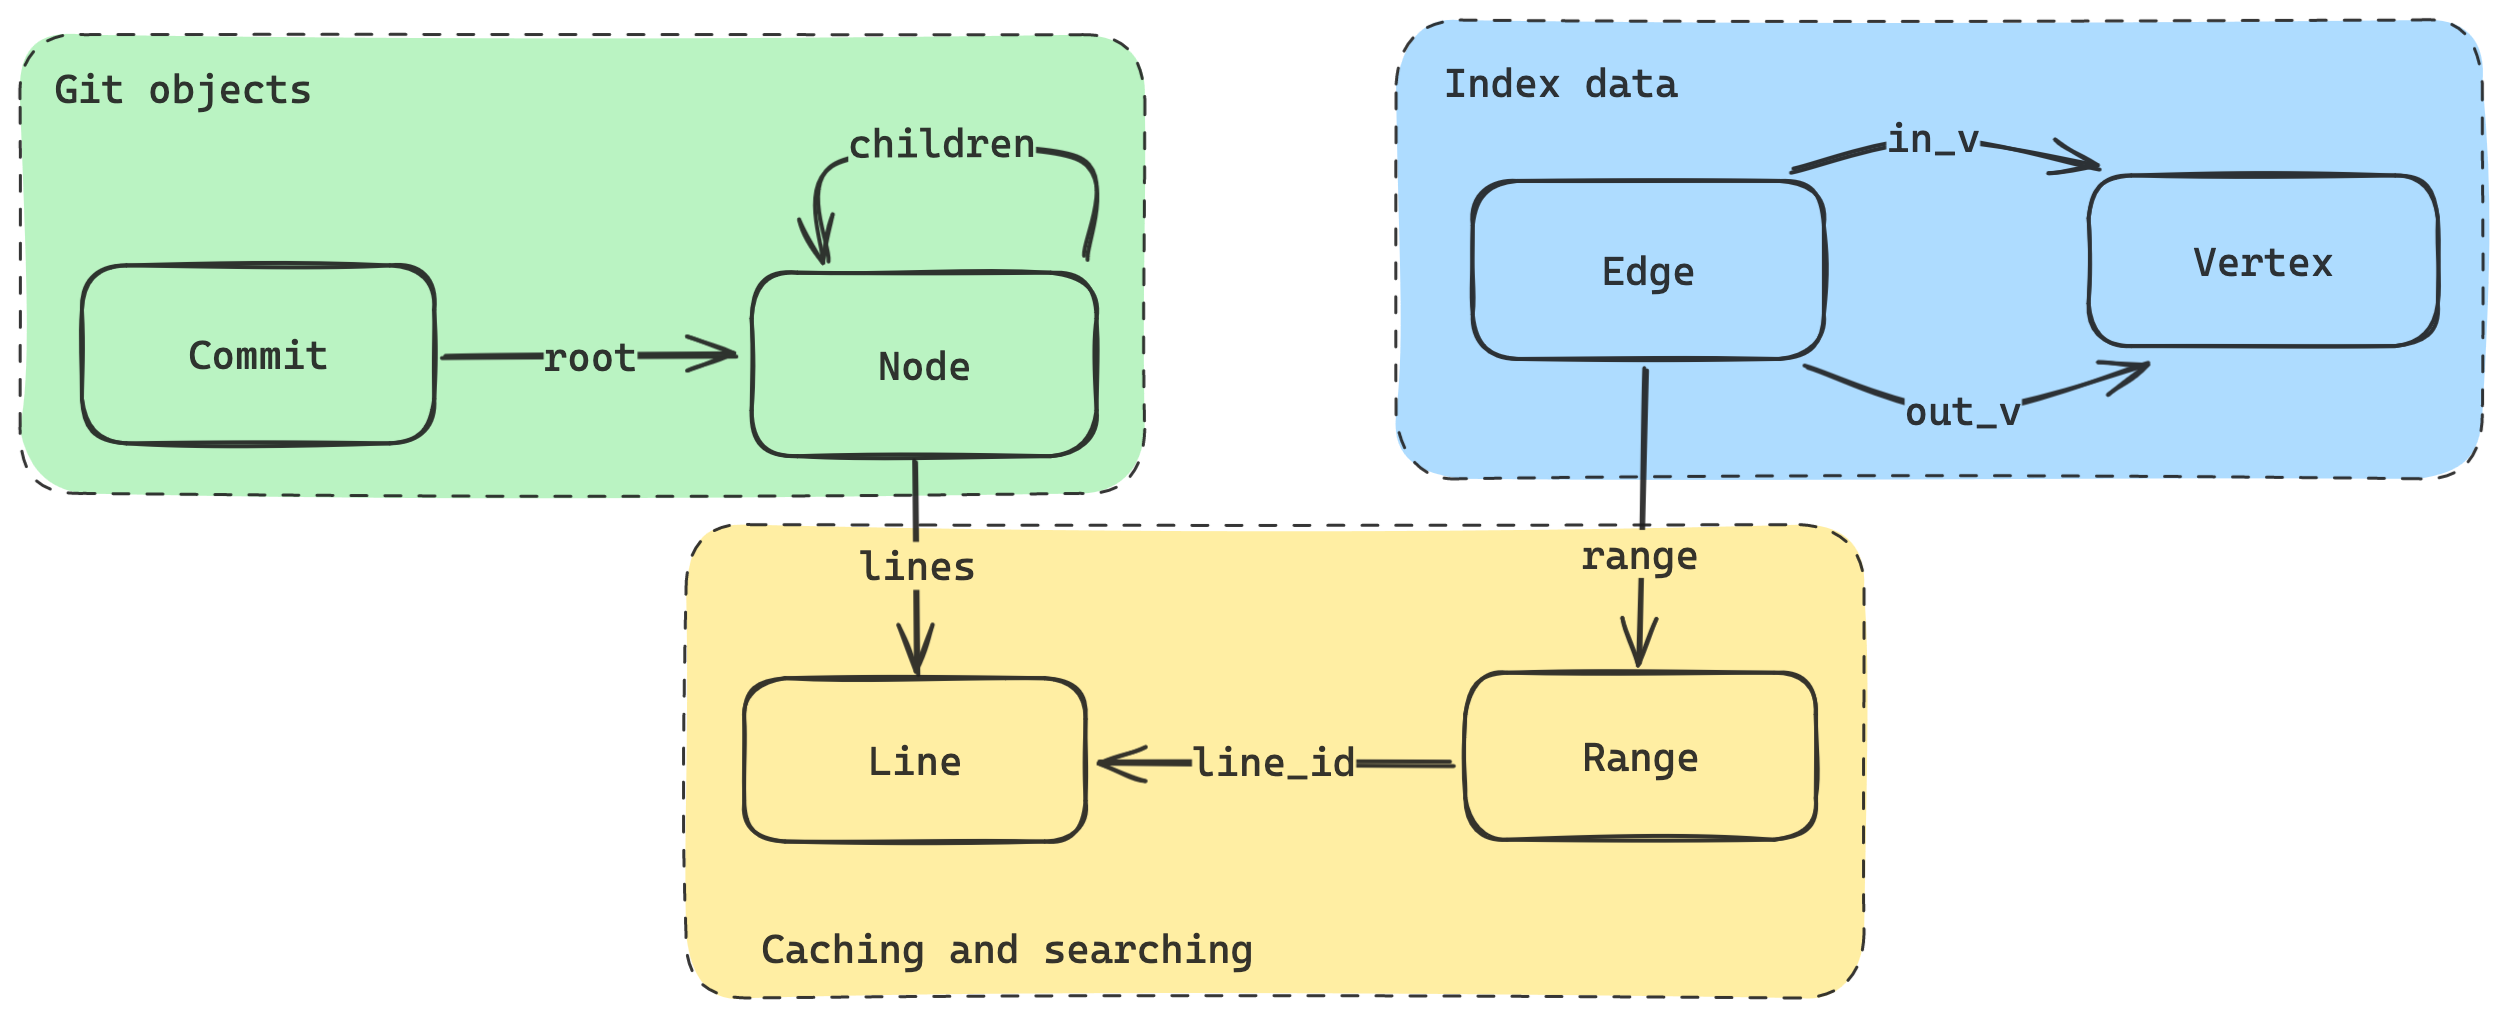
\includegraphics[width=\textwidth]{figures/model.png}

\end{frame}

\begin{frame}{\insertsection}
\framesubtitle{Данные Git-репозитория}

\begin{columns}
    \begin{column}{0.5\textwidth}
        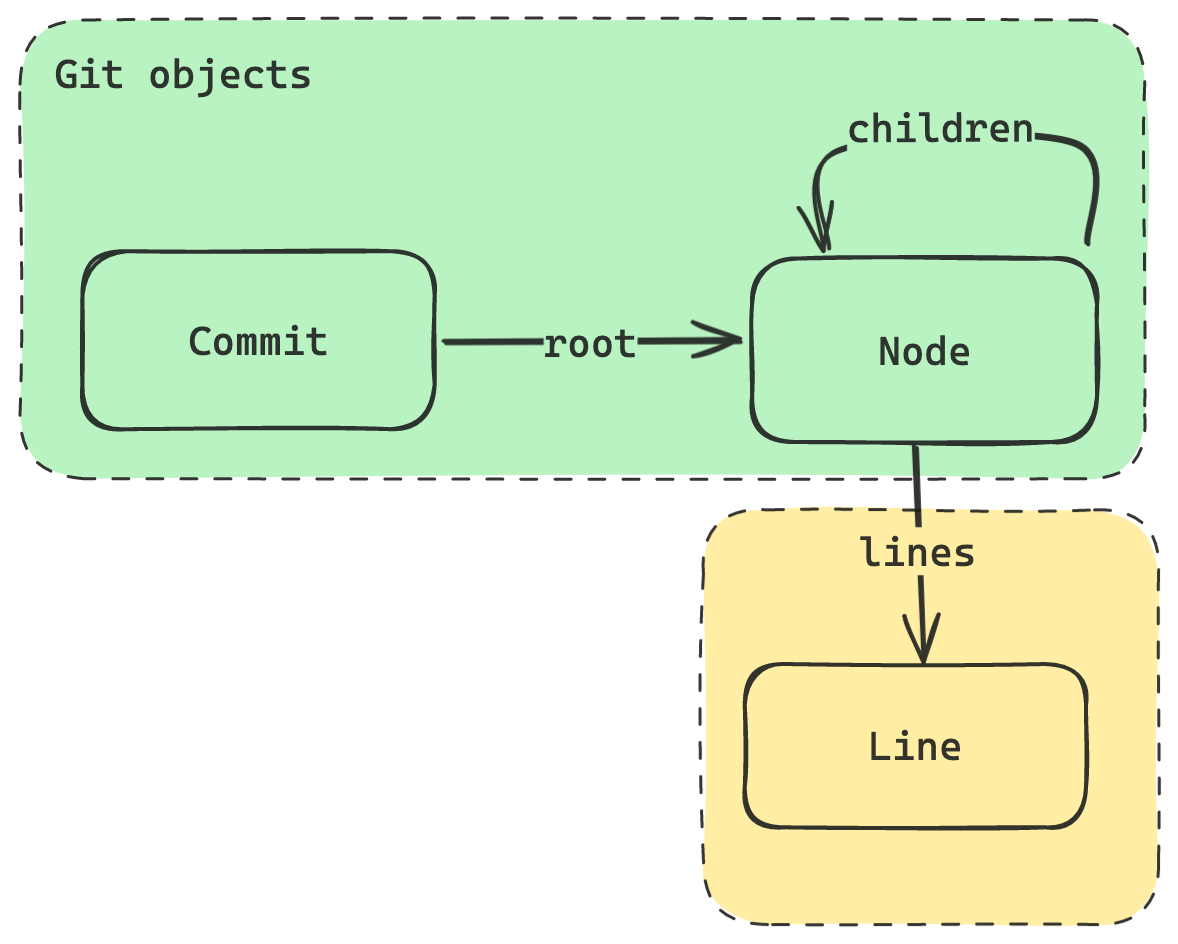
\includegraphics[width=\textwidth]{figures/model-git.png}
    \end{column}
    \begin{column}{0.5\textwidth}
        Каждый объект файла или директории в Git конвертируется и сохраняется в базу данных.\\[\baselineskip]
        
        Директории содержат список потомков (также объекты Git).\\[\baselineskip]
        
        Файлы содержат список своих строк. Каждая строка хранится отдельно, чтобы переиспользовать строки между разными версиями репозиториями и \textbf{сохранять ранее построенные индексы для неизменившихся строк}.
    \end{column}
\end{columns}

\end{frame}

\begin{frame}{\insertsection}
\framesubtitle{Данные LSIF}

\begin{columns}
    \begin{column}{0.5\textwidth}
        Граф LSIF практически как есть переносится в базу данных и представлен с помощью вершин и рёбер между ними.\\[\baselineskip]
        
        Объекты Range дополнительно выделяются в отдельную коллекцию, чтобы быстро по ним искать.\\[\baselineskip]
        
        Каждый Range хранит ссылку на строку, в которой содержится. Также они хранят полный путь к файлу, включая и коммит, на котором строился индекс.
    \end{column}
    \begin{column}{0.5\textwidth}
        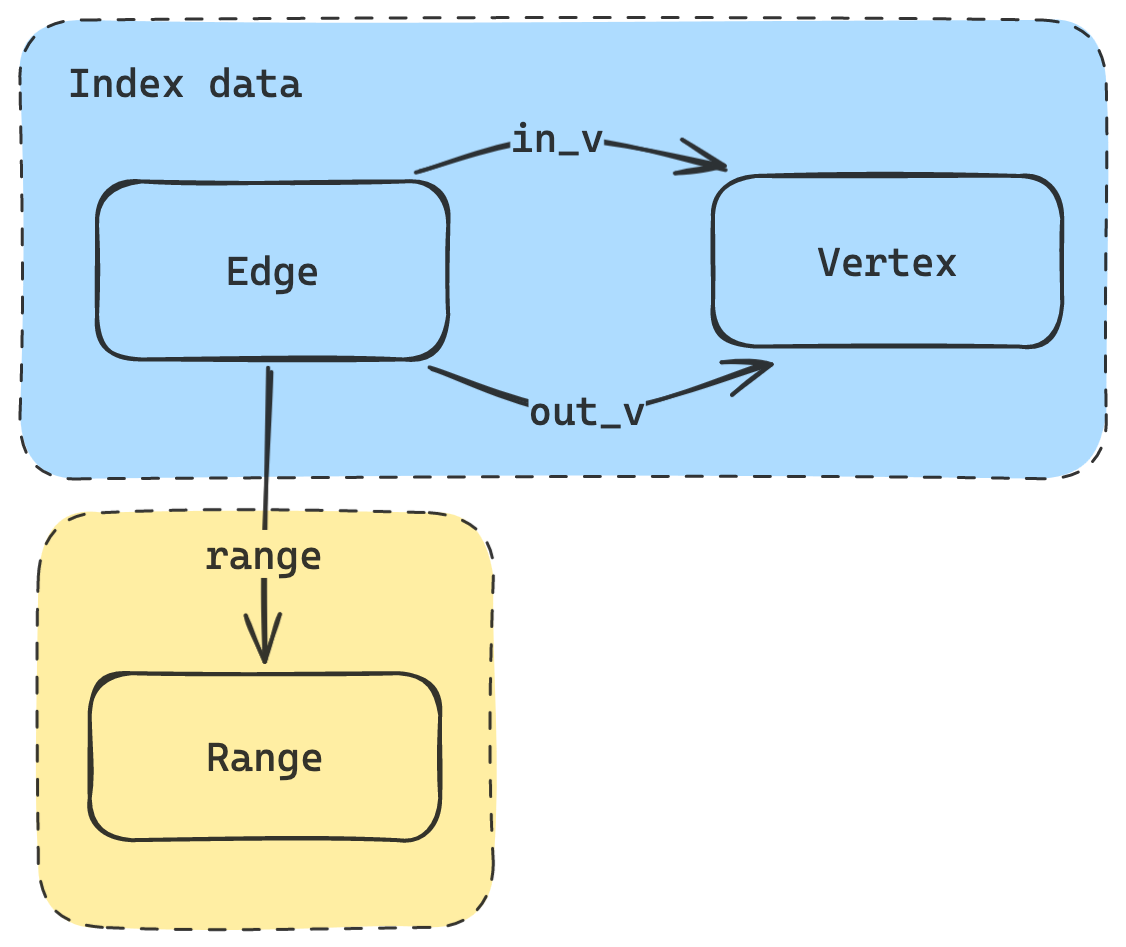
\includegraphics[width=\textwidth]{figures/model-lsif.png}
    \end{column}
\end{columns}

\end{frame}

\section{Алгоритм формирования ответа на запрос}
\begin{frame}{\insertsection}

\begin{columns}
    \begin{column}{0.5\textwidth}
        \begin{enumerate}
            \item Найти запрашиваемую подстроку в базе.
            \item Используя ребра \texttt{Next}, найти все связанные узлы \texttt{ResultSet}.
            \item Далее перейти по рёбру с типом \texttt{Definition} и найти узел, содержащий результат запроса. Ожидается найти только единственное такое ребро.
            \item \label{item-definitions} Найти ребра \texttt{Item}, соединенные с результатом запроса.
            \item Таким образом, мы нашли все подстроки, которые входят в ответ.
        \end{enumerate}
    \end{column}
    \begin{column}{0.5\textwidth}
        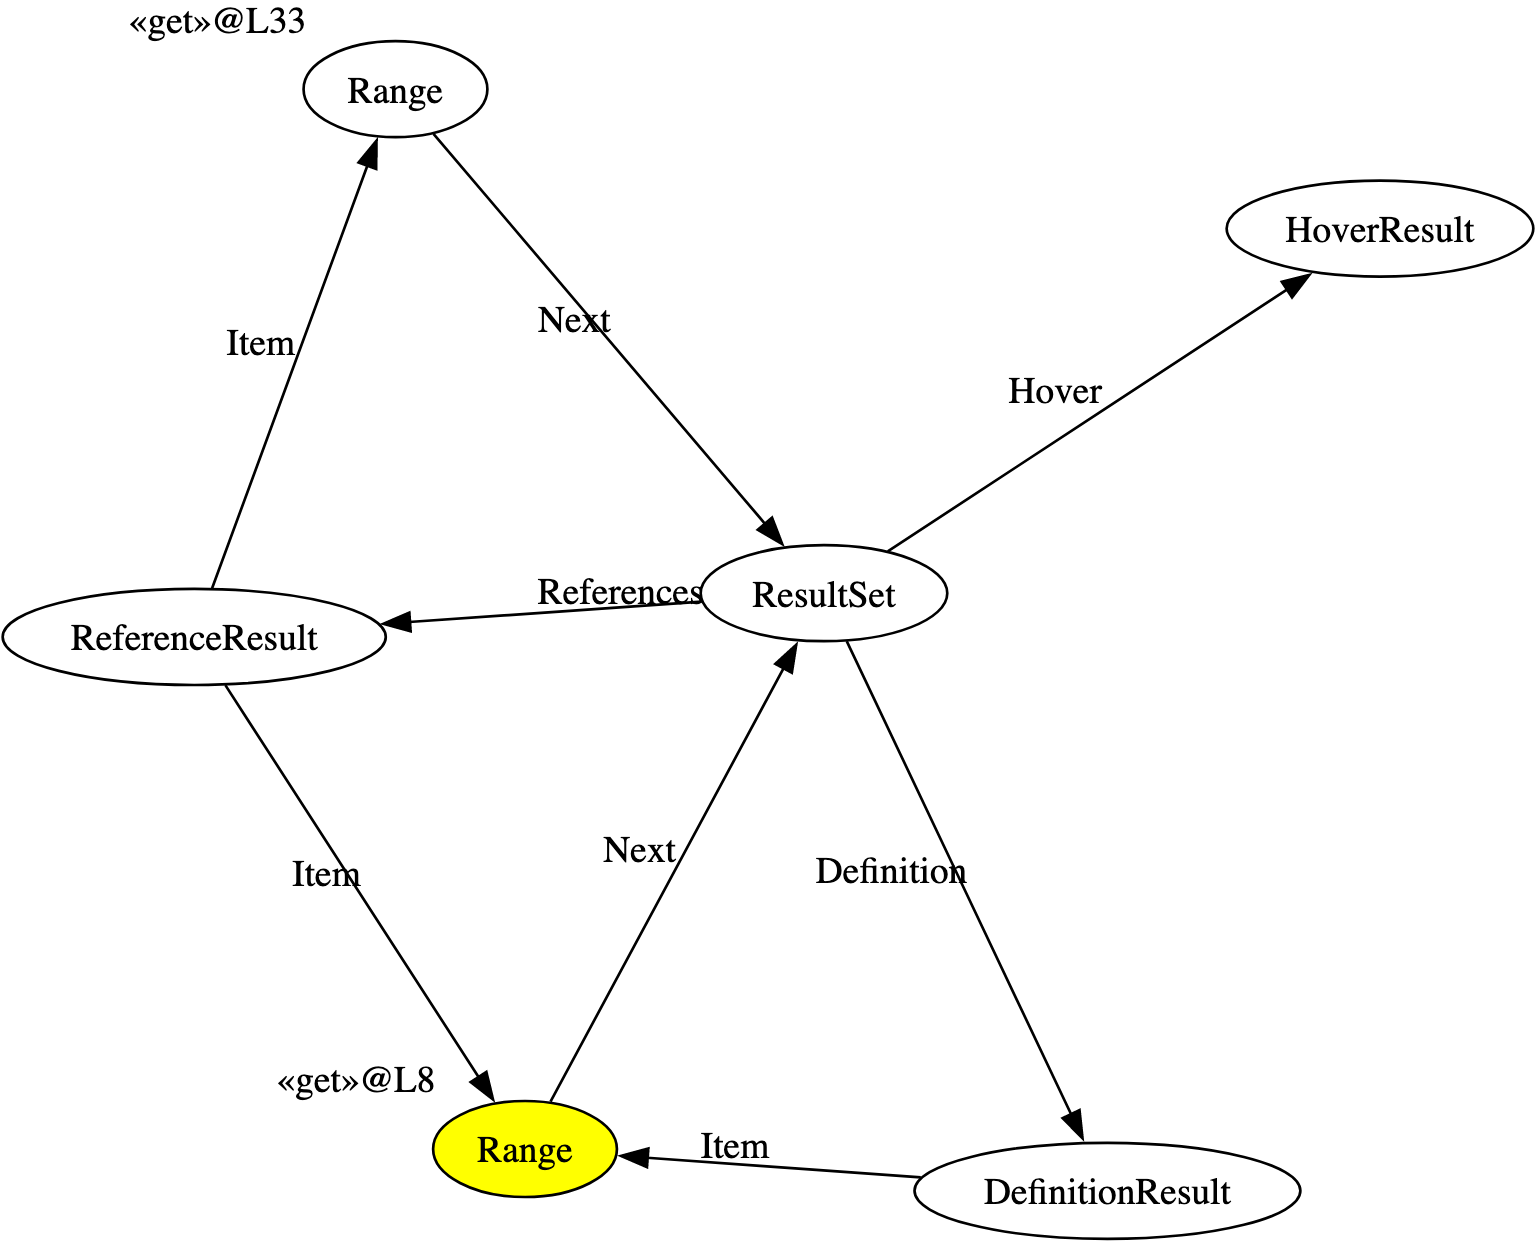
\includegraphics[width=\textwidth]{figures/lsif.png}
    \end{column}
\end{columns}
\end{frame}

\section{Технологии и инструменты реализации}
\begin{frame}{\insertsection}

Основные технологии разработки проекта:

\begin{itemize}
    \item \textbf{Rust} — язык программирования для серверной части
    \item \textbf{TypeScript} — язык программирования для пользовательского интерфейса
    \item \textbf{MongoDB} — используемая база данных
    \item \textbf{Caddyproxy} — reverse proxy для раздачи статики и передачи запросов на бекенд
    \item \textbf{JetBrains RustRover} — IDE для разработки проекта
    \item \textbf{Git} — система контроля версий
\end{itemize}

Также используются внешние библиотеки:
\begin{itemize}
    \item \textbf{vscode-web}: для упрощения сборки Visual Studio Code для веб-браузеров \\
        {\footnotesize Félix BOROT, \url{https://www.npmjs.com/package/vscode-web/v/1.82.0}}
    \item \textbf{lsp-types}: типы протокола language server для использования на серверной части \\
        {\footnotesize Gluon lang developers, \url{https://crates.io/crates/lsp-types/0.95.1}}
    \item \textbf{axum}: для написания веб-сервера и обработки запросов \\
        {\footnotesize tokio-rs developers, \url{https://crates.io/crates/axum/0.7.5}}
\end{itemize}

\end{frame}

\section{Архитектура системы}
\begin{frame}{\insertsection}

\begin{columns}
    \begin{column}{0.6\textwidth}
        Система состоит из нескольких сервисов:
        \begin{itemize}
            \item \textbf{storage} — база данных MongoDB, которая хранит все данные
            \item \textbf{indexer} — инструмент для загрузки новых данных в систему
            \item \textbf{backend} — веб-сервер, предоставляющий пользовательскому интерфейсу все необходимые API
            \item \textbf{router} — обратный прокси (Caddyproxy), позволяющий на одном адресе и раздавать файлы интерфейса, и делать запросы в бекенд
            \item \textbf{frontend} — веб-приложение в браузере пользователя на базе Visual Studio Code с использованием специально разработанного расширения
        \end{itemize}
    \end{column}
    \begin{column}{0.4\textwidth}
        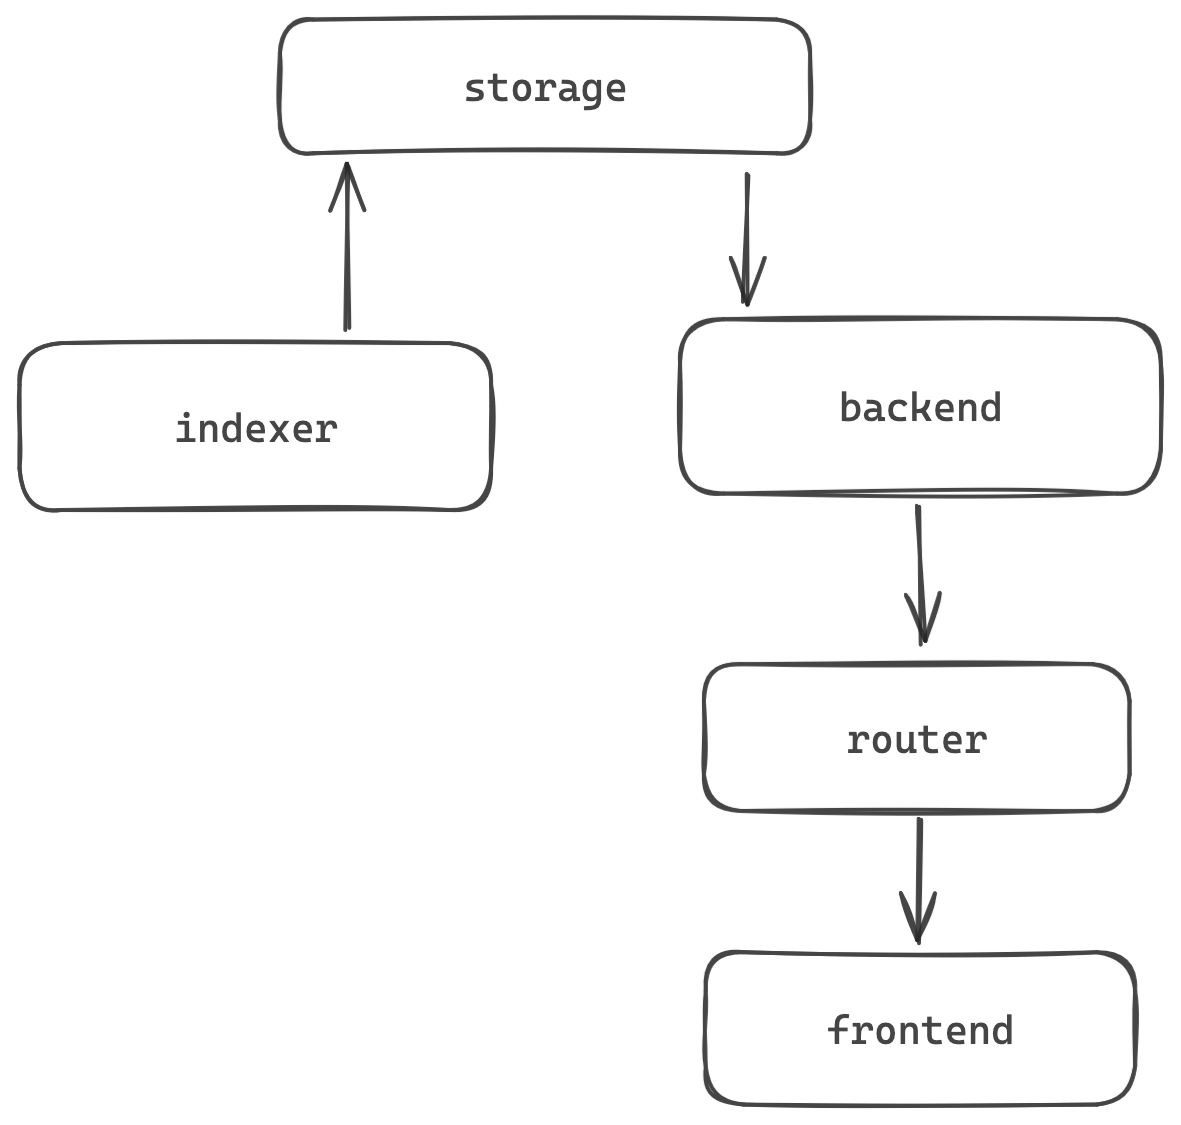
\includegraphics[width=\textwidth]{figures/architecture.png}
    \end{column}
\end{columns}

\end{frame}

\section{Входные и выходные данные}
\begin{frame}[t]{\insertsection}

\begin{columns}
    \begin{column}{0.5\textwidth}
        \textbf{Входные данные}
        \begin{itemize}
            \item Объекты Git-репозитория
            \begin{tcolorbox}%
                \texttt{%
                    .git/objects/a1/23456… \\
                    .git/objects/ff/fffff… \\
                    …
                }
            \end{tcolorbox}
            \item Результат работы LSIF-индексатора
            \begin{tcolorbox}%
                \texttt{%
                    \{``id'': 0, ``type'': ``vertex'', …\} \\
                    \{``id'': 1, ``type'': ``edge'', …\} \\
                    …
                }
            \end{tcolorbox}
        \end{itemize}
    \end{column}
    \begin{column}{0.5\textwidth}
        \textbf{Выходные данные}
        \begin{itemize}
            \item Файлы и директории репозитория
                \begin{tcolorbox}%
                    \texttt{%
                        -> GET /fs/tree/ffff…/code.c \\
                        <- \{ ``file'': \{ ... \}\} 
                    }
                \end{tcolorbox}
            \item Ответы на запросы language client (в соответствии с LSP \cite{lsp}) \\
                \begin{tcolorbox}%
                    \texttt{%
                        -> POST /lsp/textDocument/hover \\
                        <- \{ ``contents'': \{ ... \}\} 
                    }
                \end{tcolorbox}
        \end{itemize}
    \end{column}
\end{columns}

\end{frame}

\section{Основные результаты работы}
\begin{frame}[t]{\insertsection}
\framesubtitle{Справка при наведении курсора}

При наведении курсора, отображается документация по методу «\texttt{first\_entry\_async}»:

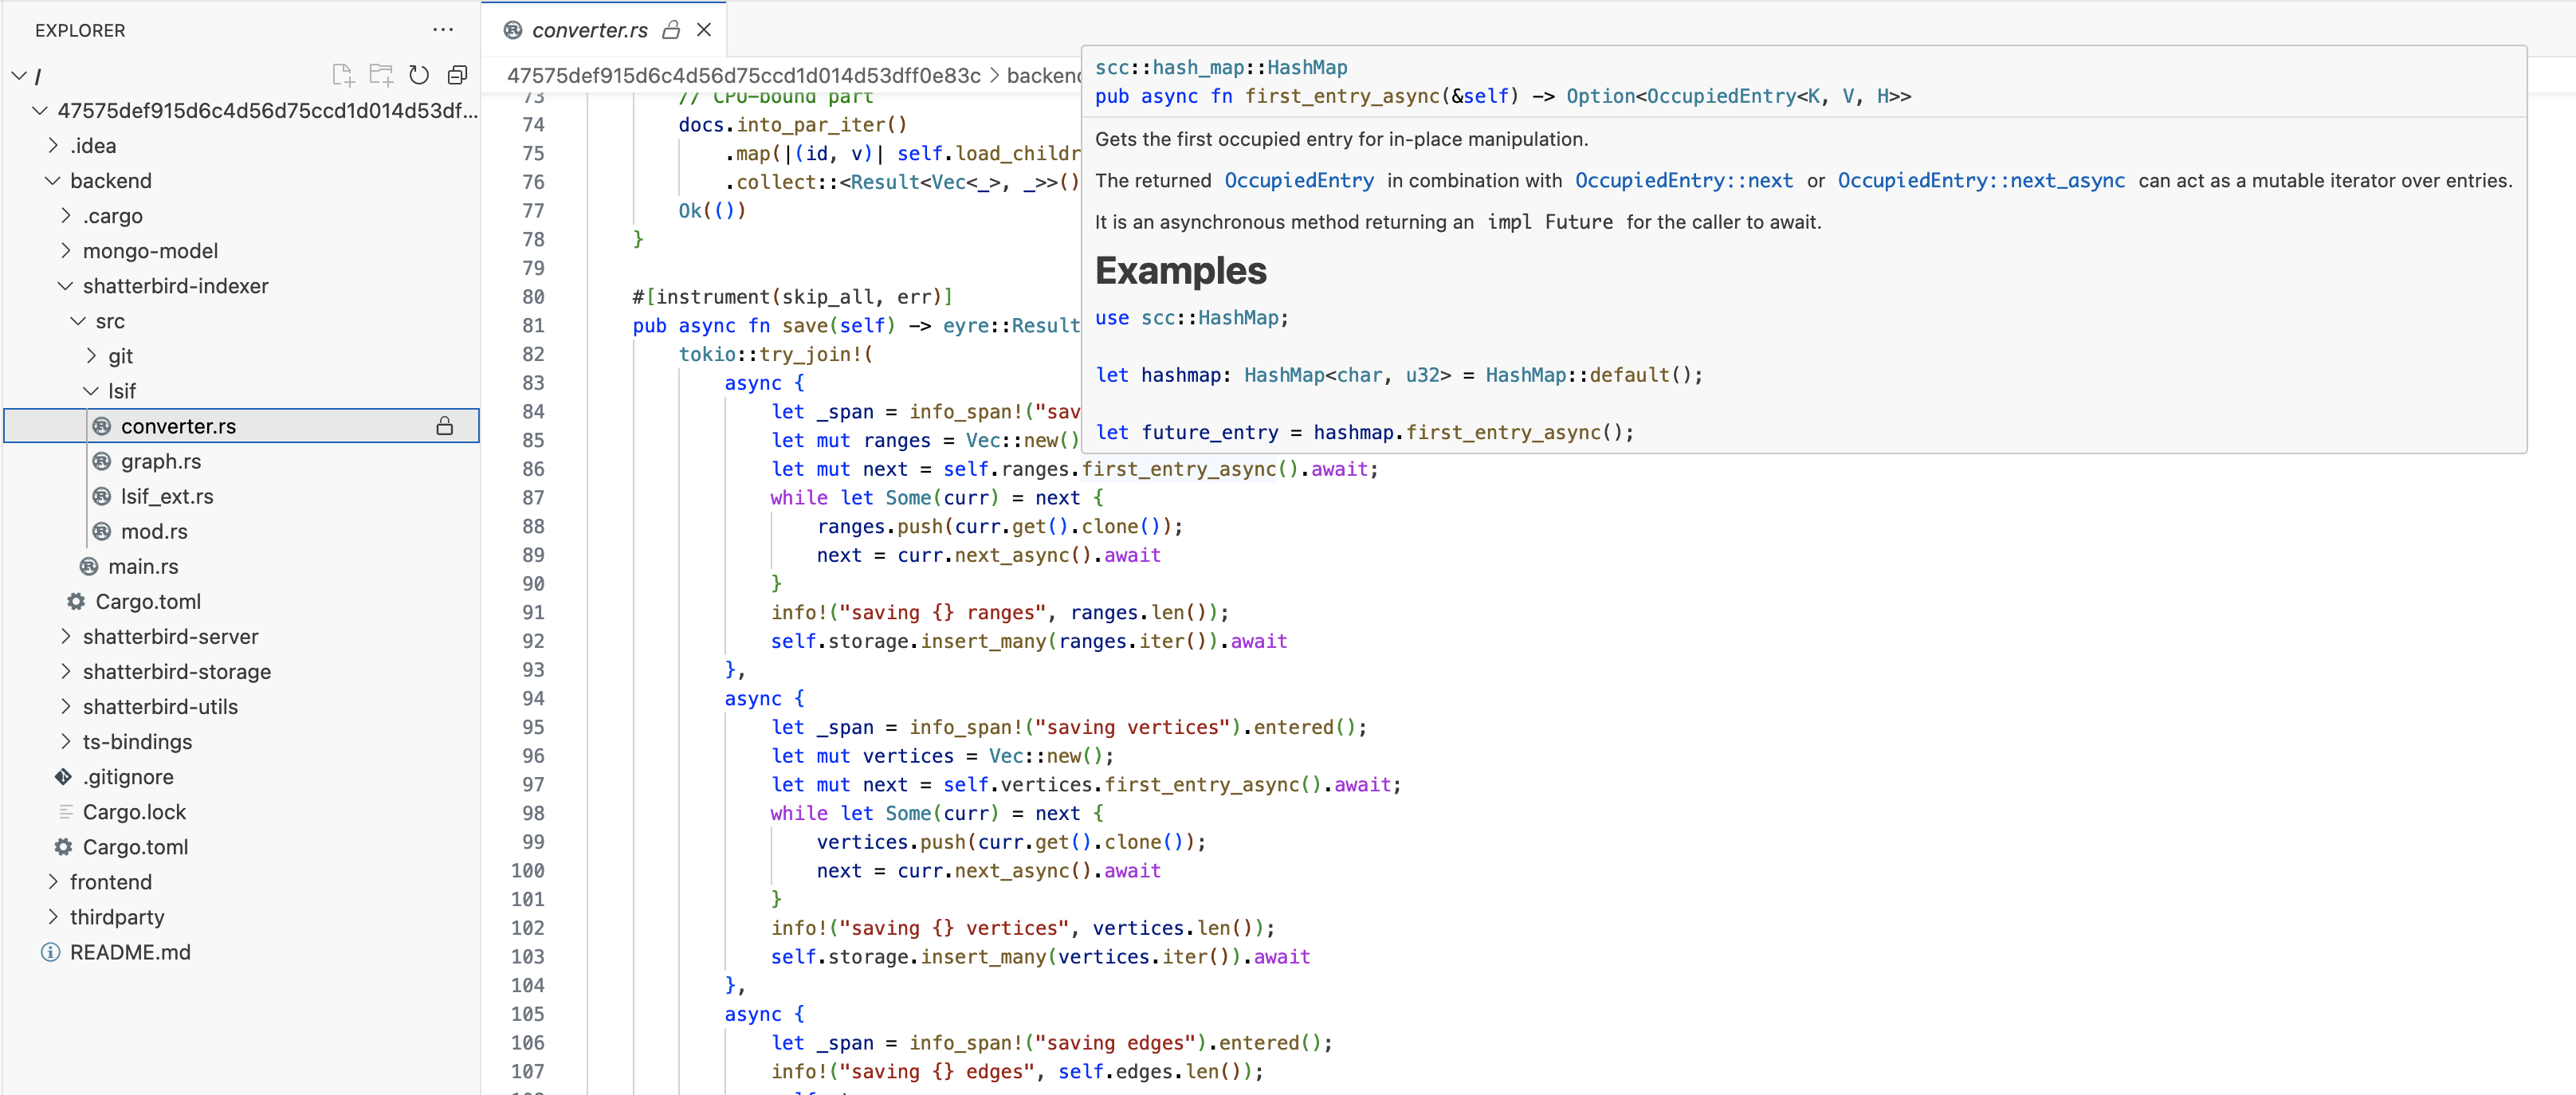
\includegraphics[width=\linewidth,keepaspectratio]{figures/demo-hover.png}

\end{frame}

\begin{frame}[t]{\insertsection}
\framesubtitle{Поиск использований символа}

Система находит все использования символа «\texttt{Range}» в репозитории:

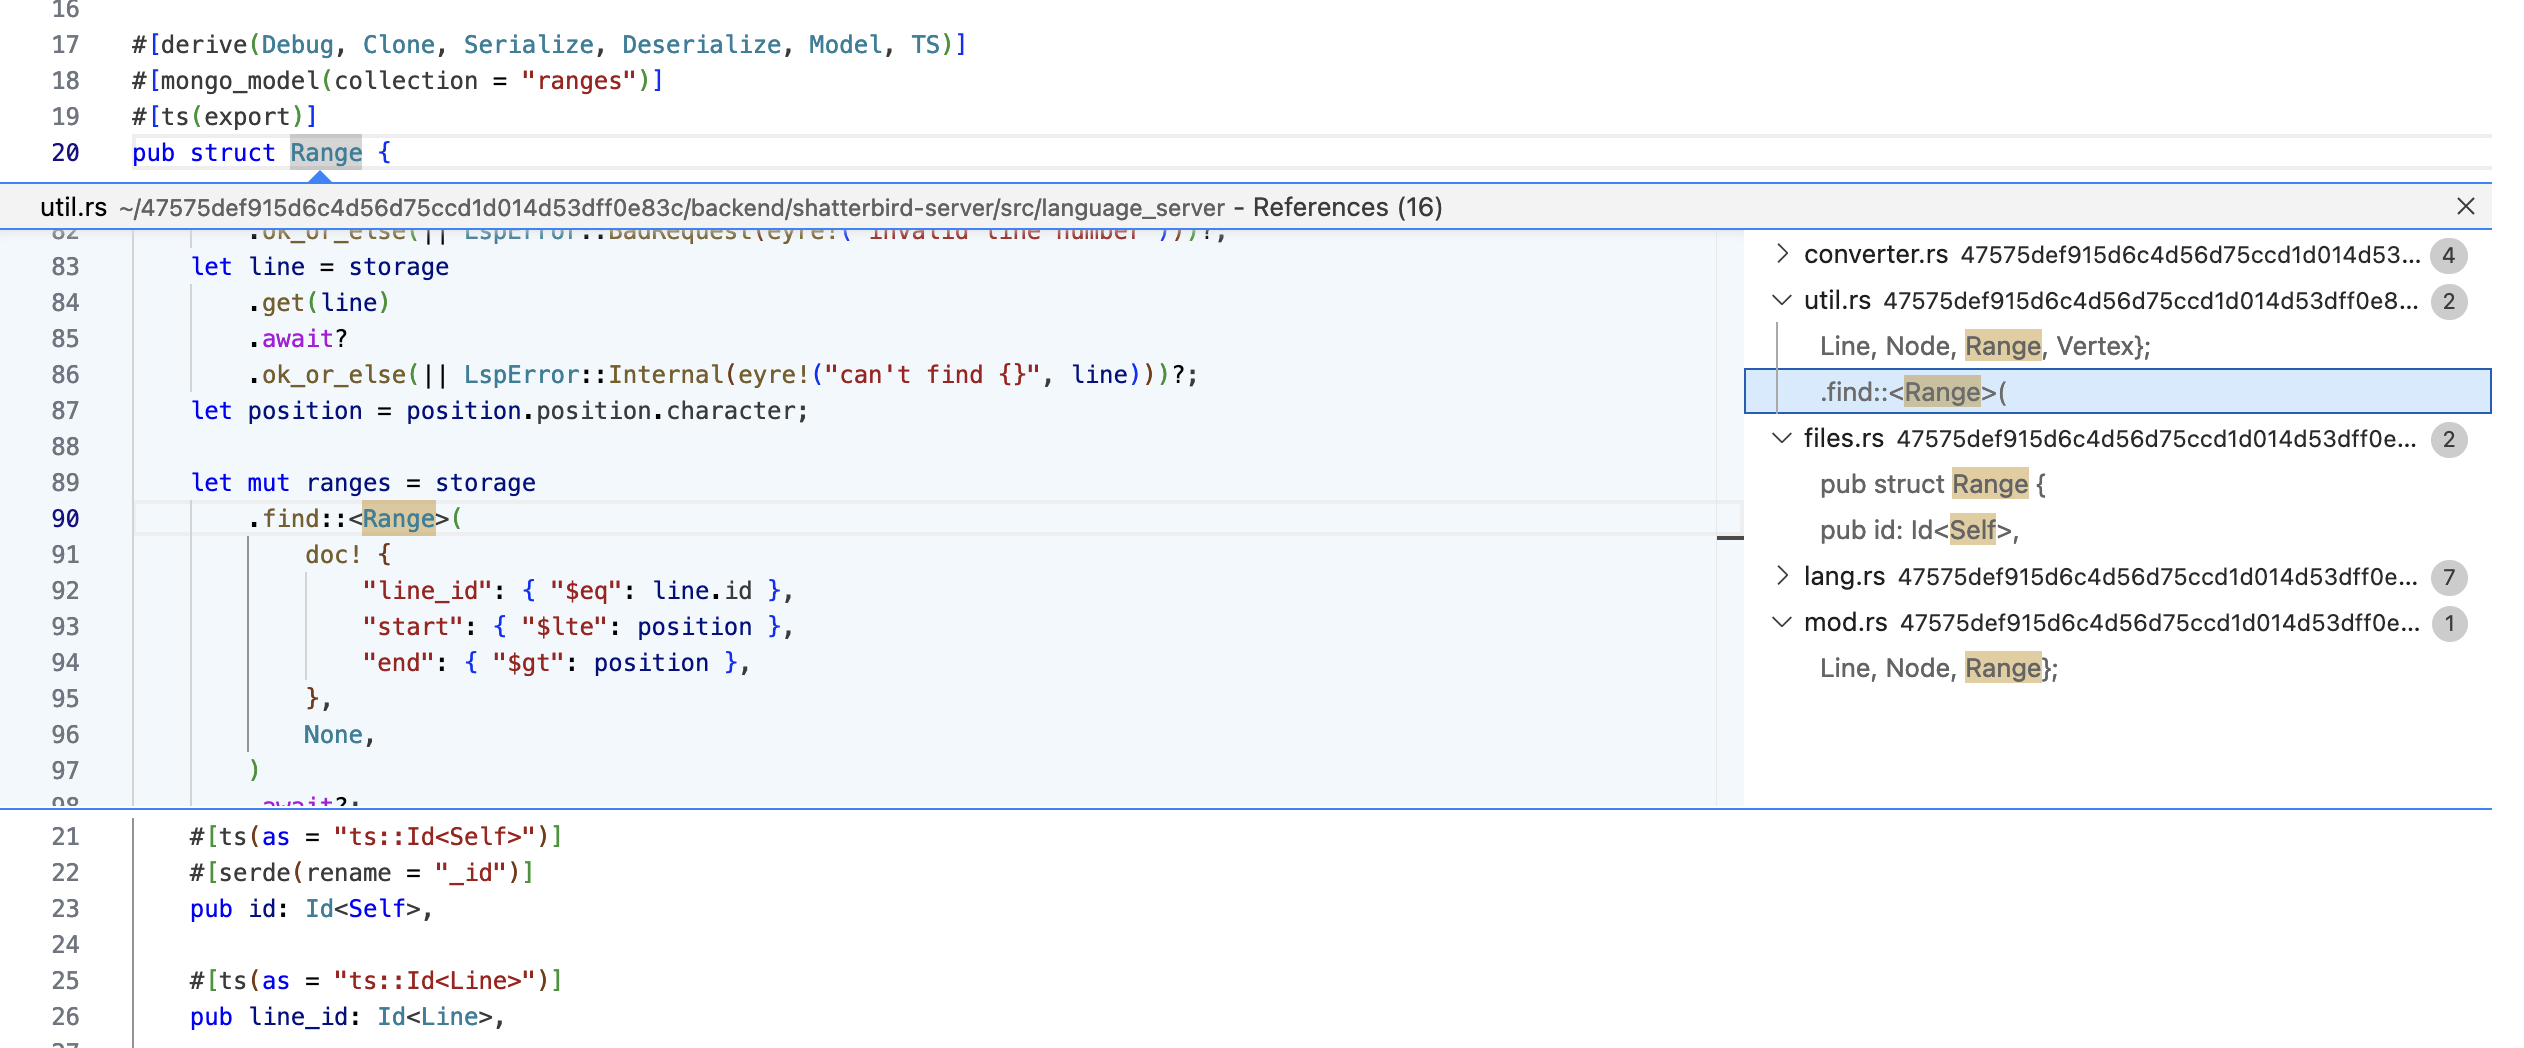
\includegraphics[width=\linewidth,keepaspectratio]{figures/demo-references.png}

\end{frame}

\begin{frame}[t]{\insertsection}
\framesubtitle{Поиск определения символа}

Система переходит к определению символа «\texttt{access}»:

\begin{columns}
    \begin{column}{0.5\textwidth}
        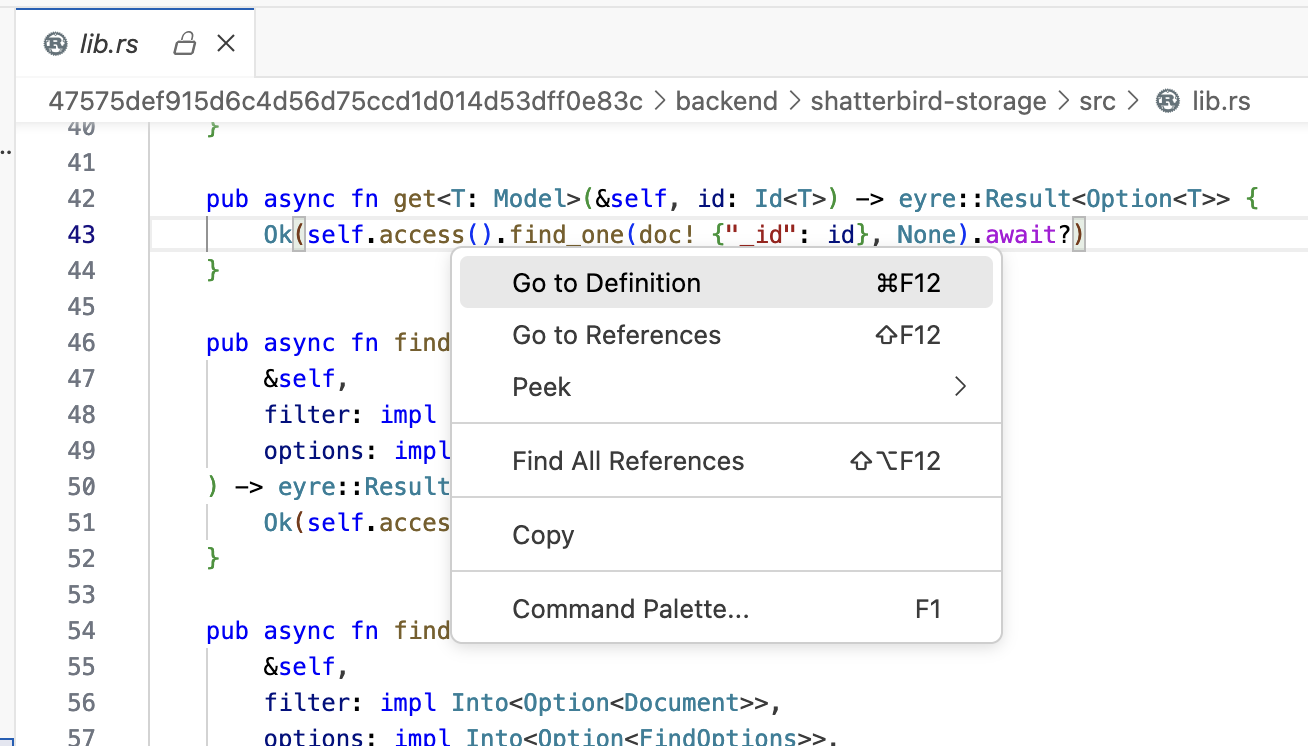
\includegraphics[width=\linewidth,keepaspectratio]{figures/demo-goto-1.png}
    \end{column}
    \begin{column}{0.5\textwidth}
        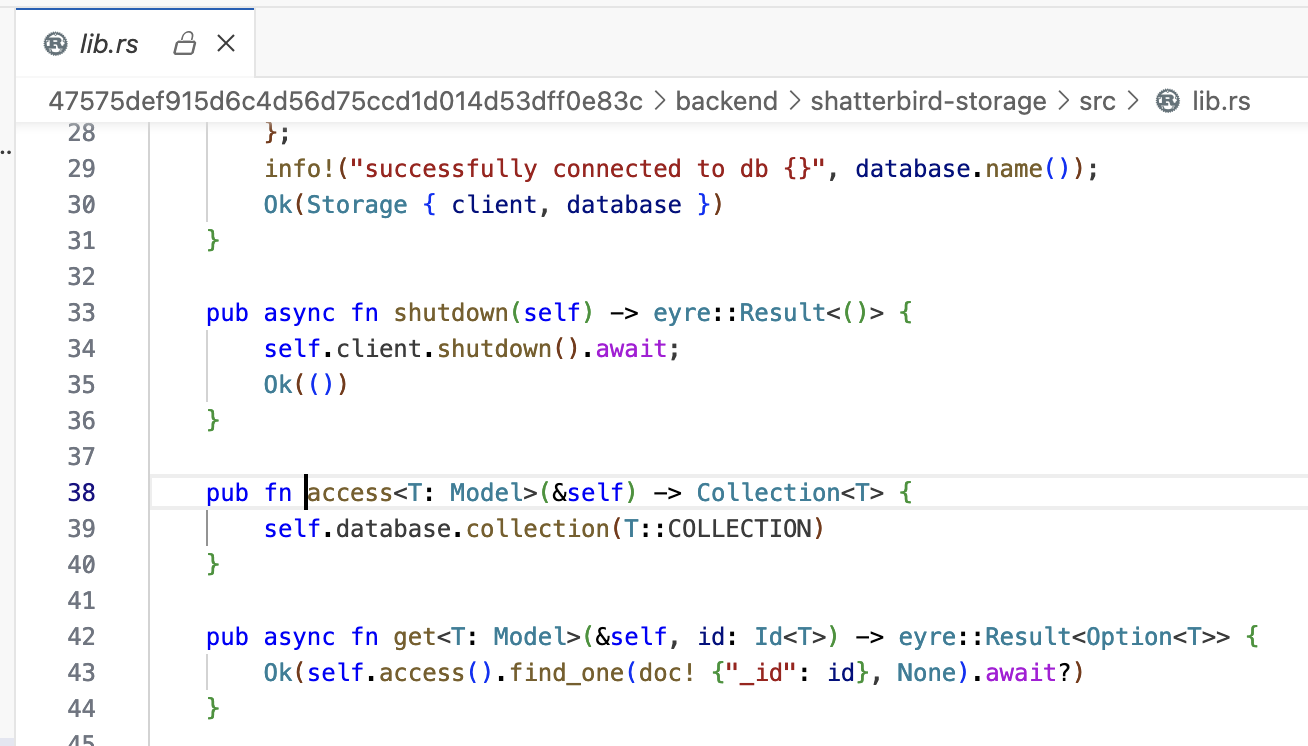
\includegraphics[width=\linewidth,keepaspectratio]{figures/demo-goto-2.png}
    \end{column}
\end{columns}

\end{frame}

\section{Пути дальнейшего развития работы}
\begin{frame}{\insertsection}
    \begin{itemize}
        \item Инструментарий для автоматизации запуска индексации;
        \item Ролевая модель и контроль доступа к отдельным репозиториям или директориям;
        \item Улучшение интеграции с Git: просмотр списка коммитов, веток, функционал «annotate»;
        \item Поддержка текстового поиска по репозиториям с поддержкой regexp;
    \end{itemize}
\end{frame}

\section{Список использованных источников}
\begin{frame}[shrink=30]{\insertsection}
    \vspace{0.5cm}
    \printbibliography
\end{frame}

\section{Спасибо за внимание}
\begingroup
\setbeamertemplate{footline}{}
\begin{frame}{\insertsection}
\centering
    \vfill Коннов Илья Александрович
    \vfill Сервис для индексирования и просмотра Git-репозиториев
    \vfill \url{https://github.com/iliakonnov/shatterbird}
    \vfill \url{iakonnov@edu.hse.ru}
    \vfill
\end{frame}
\endgroup

\end{document}